\documentclass[english,fleqn]{ieej-tec2}% documentclassの宣言で処理エンジンを指定する。fleqnは数式左寄せのため
\usepackage{amsmath,amssymb,bm}% ams-LaTeXの色々を使う
\usepackage[dvipdfmx]{graphicx,color}% 
\usepackage{nidanfloat}% 2段ぶち抜きの図を下に入れる,2段ぶち抜きの図と1段以内の図が同頁に共存するために必要
%
% 論文番号(1頁目右上にあるやつ)
% 論文番号(1頁目右上にあるやつ)
\論文番号{xx-xx-xx \par yy-yy-yy}
%
% 英語タイトル
\title{A study on the style file for IEEJ workshop.}
% 
% 著者リスト
\authorlist{%
 \authorentry*{Taro Denshi}{1}
 \authorentry{Jiro Denshi}{1}
 \authorentry{Saburo Denshi}{2}
 \authorentry{Shiro Denshi}{2}
}
% 
% 所属 [authorentryとの関連付け番号]
\affiliate[1]
 {Nihon Denki University}
\affiliate[2]
 {Nihon Electric Power Company}
%
% authormetryの番号により改行
%\breakaffiliate{1}
%\breakaffiliate{2}
%
%英文キーワード。
\begin{keyword}
Keywords, keyword2, keyword3, keyword4, keyword5, keyword6, keyword7, keyword8, keyword9, keyword10, keyword11
\end{keyword}

\begin{document}
\maketitle
%
% abstractは\begin{document}と\maketitleの間に書く
\begin{abstract}
The sentences.
\end{abstract}
%%%%%%%%%%%%%%%% ここから本文 %%%%%%%%%%%%%%%%
%
\section{Section}
Sentences

\section{Section}
Sentences

\subsection{Subsection}
Sentences\dots reference\cite{IEEJformat} reference\cite{bib2,bib3} reference\cite{bib4,bib5,bib6,bib7}

\begin{enumerate}
\item
aaaaaaaaaaaaaaaaaaaaaaaaaaaa
\item
bbbbbbbbbbbbbbbbbbbbbbbbbbbb
\end{enumerate}

\subsection{Subsection}
Sentences
%
\begin{equation}
Z = X + Y
\end{equation}
%
Sentences(No indent).
%
\begin{align}
Z &= X + Y \notag\\
& \qquad Z = X + Y \text{\scriptsize (Formula (continuing))} \\
\intertext{Explanation of the formula%
}
Z &= X + Y \times \frac AB
\end{align}

Sentence (refer to \tablename\ref{tab:example}).

\begin{table}[b]
\centering
\caption{Title.}
\label{tab:example}
\tabcolsep=1.5truemm
\begin{tabular}{|c|c|c|c|c|}\hline
Text & \hspace{4zw} &  \hspace{4zw} &  \hspace{4zw} &  \hspace{4zw} \\\hline
& & & & \\\hline
\end{tabular}
\par
\begin{minipage}{68truemm}
\scriptsize%
Explanation of the table.
\end{minipage}
\end{table}

Sentence ( refer to \tablename\ref{tab:nidanfloat:example})

\begin{table*}[t]
\centering
\caption{Title.}
\label{tab:nidanfloat:example}
\tabcolsep=1.5truemm
\begin{tabular}{|c|c|c|c|c|c|c|c|c|c|c|}\hline
Text & \hspace{4zw} &  \hspace{4zw} &  \hspace{4zw} &  \hspace{4zw} &  \hspace{4zw} &  \hspace{4zw} &  \hspace{4zw} &  \hspace{4zw} &  \hspace{4zw} &  \hspace{4zw} \\\hline
& & & & & & & & & & \\\hline
\end{tabular}
\par
% 図表説明の入れ方がハードコーディングなのはご愛嬌
\begin{minipage}{\hsize}
\scriptsize\centering%
Explanation of the table (centering).
\end{minipage}
\end{table*}

Sentence (refer to \figurename\ref{fig:example}).

%% 貼るためのeps画像をtexから作成 %%
\bgroup
\catcode37=11
\gdef\percentcharacter{%}
\egroup
\newwrite\fout%
\immediate\openout\fout=ieejtec2figure.eps%
\immediate\write\fout{\percentcharacter !PS-Adobe-3.0 EPSF-3.0}%
\immediate\write\fout{\percentcharacter\percentcharacter BoundingBox: 0 0 100 60}%
\immediate\write\fout{gsave}%
\immediate\write\fout{1 setlinewidth}%
\immediate\write\fout{gsave 0.75 setgray 0.25 setlinewidth}%
\immediate\write\fout{newpath 0 15 moveto 100 0 rlineto stroke}%
\immediate\write\fout{newpath 0 30 moveto 100 0 rlineto stroke}%
\immediate\write\fout{newpath 0 45 moveto 100 0 rlineto stroke}%
\immediate\write\fout{grestore}%
\immediate\write\fout{newpath 0 0 moveto 100 50 lineto stroke}%
\immediate\write\fout{newpath 100 0 moveto 0 0 lineto 0 60 lineto stroke}%
\immediate\write\fout{grestore}%
\immediate\write\fout{\percentcharacter\percentcharacter EOF}%
\immediate\closeout\fout%
%% ここまで %%

\begin{figure}[b]
\centering
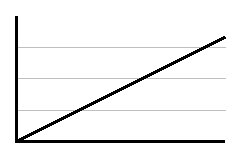
\includegraphics[width=70truemm]{ieejtec2figure.eps}
\par
(a) Graph 1.
\caption{Title.}
\label{fig:example}
\end{figure}


Sentence.

qwertyuiop
asdfghjkl
zxcvbnm
qwertyuiop
asdfghjkl
zxcvbnm
qwertyuiop
asdfghjkl
zxcvbnm
qwertyuiop
asdfghjkl
zxcvbnm
qwertyuiop
asdfghjkl
zxcvbnm
qwertyuiop
asdfghjkl
zxcvbnm
qwertyuiop
asdfghjkl
zxcvbnm
\begin{thebibliography}{99}
\bibitem{IEEJformat}
\verb|http://www.iee.jp/?page_id=4843|
\bibitem{bib2}
Name : “Title English”, Name of journal, Vol., No. p.000 (issued year)
\bibitem{bib3}
Name and Name : “Title English”, Name of journal, Vol., No. p.000 (issued year)
\bibitem{bib4}
Name : “Title English”, Name of journal, Vol., No. p.000 (issued year)
\bibitem{bib5}
Name : “Title English”, Name of journal, Vol., No. p.000 (issued year)
\bibitem{bib6}
Name : “Title English”, Name of journal, Vol., No. p.000 (issued year)
\bibitem{bib7}
Name : “Title English”, Name of journal, Vol., No. p.000 (issued year)
\bibitem{bib8}
Name : “Title English”, Name of journal, Vol., No. p.000 (issued year)
\bibitem{bib9}
Name : “Title English”, Name of journal, Vol., No. p.000 (issued year)
\bibitem{bib10}
Name : “Title English”, Name of journal, Vol., No. p.000 (issued year)
\bibitem{bib11}
Name : “Title English”, Name of journal, Vol., No. p.000 (issued year)
\end{thebibliography}


\end{document}